\tikzstyle{state}=[shape=circle,draw=blue!50,fill=blue!20]
\tikzstyle{lightedge}=[<-,dotted]
\tikzstyle{mainstate}=[state,thick]
\tikzstyle{mainedge}=[<-,thick]

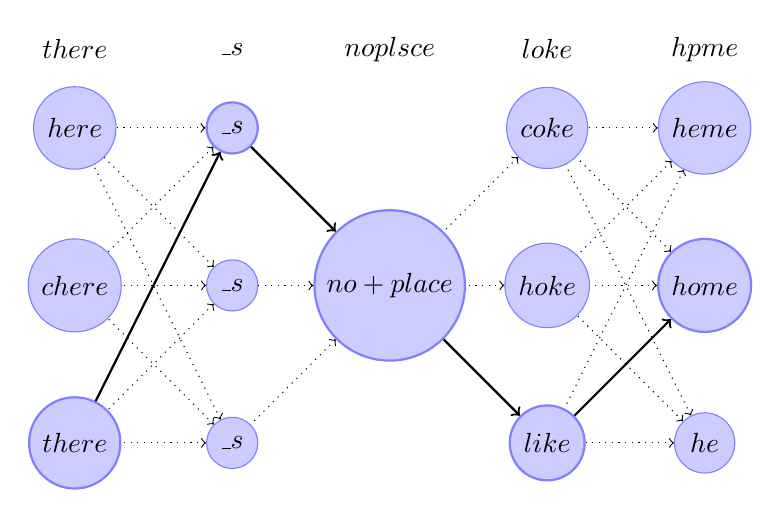
\begin{tikzpicture}[]
% 1st column
\node               at (0,6) {$there$};
\node[state] (s1_1) at (0,5) {$here$};
\node[state] (s2_1) at (0,3) {$chere$};
\node[mainstate] (s3_1) at (0,1) {$there$};
% 2nd column
\node               at (2,6) {$\_s$};
\node[mainstate] (s1_2) at (2,5) {$\_s$}
    edge[lightedge] (s1_1)
    edge[lightedge] (s2_1)
    edge[mainedge] (s3_1);
\node[state] (s2_2) at (2,3) {$\_s$}
    edge[lightedge] (s1_1)
    edge[lightedge] (s2_1)
    edge[lightedge] (s3_1);
\node[state] (s3_2) at (2,1) {$\_s$}
    edge[lightedge] (s1_1)
    edge[lightedge] (s2_1)
    edge[lightedge] (s3_1);
% 3rd column
\node               at (4,6) {$noplsce$};
\node[mainstate] (s2_3) at (4,3) {$no+place$}
    edge[mainedge] (s1_2)
    edge[lightedge] (s2_2)
    edge[lightedge] (s3_2);

% 4th column
\node               at (6,6) {$loke$};
\node[state] (s4_1) at (6,5) {$coke$}
    edge[lightedge] (s2_3);
\node[state] (s4_2) at (6,3) {$hoke$}
    edge[lightedge] (s2_3);
\node[mainstate] (s4_3) at (6,1) {$like$}
    edge[mainedge] (s2_3);
    
% 5th column
\node               at (8,6) {$hpme$};
\node[state] (s5_2) at (8,5) {$heme$}
    edge[lightedge] (s4_1)
    edge[lightedge] (s4_2)
    edge[lightedge] (s4_3);
\node[mainstate] (s2_2) at (8,3) {$home$}
    edge[lightedge] (s4_1)
    edge[lightedge] (s4_2)
    edge[mainedge] (s4_3);
\node[state] (s3_2) at (8,1) {$he$}
    edge[lightedge] (s4_1)
    edge[lightedge] (s4_2)
    edge[lightedge] (s4_3);

\end{tikzpicture}
